% Options for packages loaded elsewhere
% Options for packages loaded elsewhere
\PassOptionsToPackage{unicode}{hyperref}
\PassOptionsToPackage{hyphens}{url}
\PassOptionsToPackage{dvipsnames,svgnames,x11names}{xcolor}
%
\documentclass[twoside]{extreport}
\usepackage{report-generic}
\usepackage{report-language}
% Alter some LaTeX defaults for better treatment of figures:
% See p.105 of "TeX Unbound" for suggested values.
% See pp. 199-200 of Lamport's "LaTeX" book for details.
%   General parameters, for ALL pages:
\renewcommand{\topfraction}{0.9}	% max fraction of floats at top
\renewcommand{\bottomfraction}{0.8}	% max fraction of floats at bottom
%   Parameters for TEXT pages (not float pages):
\setcounter{topnumber}{2}
\setcounter{bottomnumber}{2}
\setcounter{totalnumber}{4}     % 2 may work better
\setcounter{dbltopnumber}{2}    % for 2-column pages
\renewcommand{\dbltopfraction}{0.9}	% fit big float above 2-col. text
\renewcommand{\textfraction}{0.07}	% allow minimal text w. figs
%   Parameters for FLOAT pages (not text pages):
\renewcommand{\floatpagefraction}{0.7}	% require fuller float pages
% N.B.: floatpagefraction MUST be less than topfraction !!
\renewcommand{\dblfloatpagefraction}{0.7}	% require fuller float pages
\pagenumbering{arabic}


\title{Methodologie van het vernieuwd Meetnet Algemene
Broedvogelmonitoring Vlaanderen (ABV2.0)}
\citationtitle{Methodologie van het vernieuwd Meetnet Algemene
Broedvogelmonitoring Vlaanderen (ABV2.0)}
\titleauthor{Stijn Vandenbulcke, Thierry Onckelinx}
\displaycolophon{1}
\colophonauthor{Stijn Vandenbulcke, Thierry Onckelinx}
\colophonauthortag{Auteurs}
\reviewer{TBD TBD}
\reviewertag{Reviewers}
\missiontag{Het INBO is het onderzoeksinstituut van de Vlaamse overheid
dat via onafhankelijk toegepast wetenschappelijk onderzoek, data- en
kennisontsluiting het biodiversiteitsbeleid en -beheer onderbouwt en
evalueert.}
\entityname{Instituut voor Natuur- en Bosonderzoek}
\entityaddress{INBO Brussel, Herman Teirlinckgebouw, Havenlaan 88 bus
73, 1000 Brussel}
\locationtag{Vestiging}
\tagline{vlaanderen-wetenschap.pdf}
\definecolours{inbo}
\entityurl{https://www.vlaanderen.be/inbo}
\entityurltext{vlaanderen.be/inbo}
\pagefootmessage{!!! missing flandersqmd.doi !!!}
\public{1}
\corresponding{\href{mailto:info@inbo.be}{info@inbo.be} }
\country{België}
\citationtag{Wijze van citeren}
\shortauthor{ Vandenbulcke, S. \& Onckelinx, T.}
\citationyear{2026}
\reportnr{I}
\seriestag{Rapporten van het}
\iseriestag{Interne rapporten van het}
\city{Brussel}
\issn{1782-9054}
\vu{Verantwoordelijke uitgever}
\vuname{Hilde Eggermont}
\covertag{Foto cover}
\client{}
\cooperation{}
\ccby{Dit werk valt onder een \href{https://creativecommons.org/licenses/by/4.0/}{Creative Commons Naamsvermelding 4.0 Internationaal-licentie}.}
\titlelogo{
\includegraphics[height = 17mm, keepaspectratio]{inbo-logo.pdf}}




\usepackage{xcolor}
\usepackage{amsmath,amssymb}
\setcounter{secnumdepth}{5}
\usepackage{iftex}
\ifPDFTeX
  \usepackage[T1]{fontenc}
  \usepackage[utf8]{inputenc}
  \usepackage{textcomp} % provide euro and other symbols
\else % if luatex or xetex
  \usepackage{unicode-math} % this also loads fontspec
  \defaultfontfeatures{Scale=MatchLowercase}
  \defaultfontfeatures[\rmfamily]{Ligatures=TeX,Scale=1}
\fi
\usepackage{lmodern}
\ifPDFTeX\else
  % xetex/luatex font selection
  \setmainfont[]{Calibri}
  \setmonofont[]{Inconsolatazi4}
\fi
% Use upquote if available, for straight quotes in verbatim environments
\IfFileExists{upquote.sty}{\usepackage{upquote}}{}
\IfFileExists{microtype.sty}{% use microtype if available
  \usepackage[]{microtype}
  \UseMicrotypeSet[protrusion]{basicmath} % disable protrusion for tt fonts
}{}
\makeatletter
\@ifundefined{KOMAClassName}{% if non-KOMA class
  \IfFileExists{parskip.sty}{%
    \usepackage{parskip}
  }{% else
    \setlength{\parindent}{0pt}
    \setlength{\parskip}{6pt plus 2pt minus 1pt}}
}{% if KOMA class
  \KOMAoptions{parskip=half}}
\makeatother
% Make \paragraph and \subparagraph free-standing
\makeatletter
\ifx\paragraph\undefined\else
  \let\oldparagraph\paragraph
  \renewcommand{\paragraph}{
    \@ifstar
      \xxxParagraphStar
      \xxxParagraphNoStar
  }
  \newcommand{\xxxParagraphStar}[1]{\oldparagraph*{#1}\mbox{}}
  \newcommand{\xxxParagraphNoStar}[1]{\oldparagraph{#1}\mbox{}}
\fi
\ifx\subparagraph\undefined\else
  \let\oldsubparagraph\subparagraph
  \renewcommand{\subparagraph}{
    \@ifstar
      \xxxSubParagraphStar
      \xxxSubParagraphNoStar
  }
  \newcommand{\xxxSubParagraphStar}[1]{\oldsubparagraph*{#1}\mbox{}}
  \newcommand{\xxxSubParagraphNoStar}[1]{\oldsubparagraph{#1}\mbox{}}
\fi
\makeatother


\usepackage{longtable,booktabs,array}
\newcounter{none} % for unnumbered tables
\usepackage{calc} % for calculating minipage widths
% Correct order of tables after \paragraph or \subparagraph
\usepackage{etoolbox}
\makeatletter
\patchcmd\longtable{\par}{\if@noskipsec\mbox{}\fi\par}{}{}
\makeatother
% Allow footnotes in longtable head/foot
\IfFileExists{footnotehyper.sty}{\usepackage{footnotehyper}}{\usepackage{footnote}}
\makesavenoteenv{longtable}
\usepackage{graphicx}
\makeatletter
\newsavebox\pandoc@box
\newcommand*\pandocbounded[1]{% scales image to fit in text height/width
  \sbox\pandoc@box{#1}%
  \Gscale@div\@tempa{\textheight}{\dimexpr\ht\pandoc@box+\dp\pandoc@box\relax}%
  \Gscale@div\@tempb{\linewidth}{\wd\pandoc@box}%
  \ifdim\@tempb\p@<\@tempa\p@\let\@tempa\@tempb\fi% select the smaller of both
  \ifdim\@tempa\p@<\p@\scalebox{\@tempa}{\usebox\pandoc@box}%
  \else\usebox{\pandoc@box}%
  \fi%
}
% Set default figure placement to htbp
\def\fps@figure{htbp}
\makeatother



\ifLuaTeX
\usepackage[bidi=basic,shorthands=off]{babel}
\else
\usepackage[bidi=default,shorthands=off]{babel}
\fi
\ifPDFTeX
\else
\babelfont{rm}[]{Calibri}
\fi
\ifLuaTeX
  \usepackage{selnolig} % disable illegal ligatures
\fi


\setlength{\emergencystretch}{3em} % prevent overfull lines

\providecommand{\tightlist}{%
  \setlength{\itemsep}{0pt}\setlength{\parskip}{0pt}}



 


\makeatletter
\@ifpackageloaded{bookmark}{}{\usepackage{bookmark}}
\makeatother
\makeatletter
\@ifpackageloaded{caption}{}{\usepackage{caption}}
\AtBeginDocument{%
\ifdefined\contentsname
  \renewcommand*\contentsname{Inhoudsopgave}
\else
  \newcommand\contentsname{Inhoudsopgave}
\fi
\ifdefined\listfigurename
  \renewcommand*\listfigurename{Lijst van figuren}
\else
  \newcommand\listfigurename{Lijst van figuren}
\fi
\ifdefined\listtablename
  \renewcommand*\listtablename{Lijst van tabellen}
\else
  \newcommand\listtablename{Lijst van tabellen}
\fi
\ifdefined\figurename
  \renewcommand*\figurename{Figuur}
\else
  \newcommand\figurename{Figuur}
\fi
\ifdefined\tablename
  \renewcommand*\tablename{Tabel}
\else
  \newcommand\tablename{Tabel}
\fi
}
\@ifpackageloaded{float}{}{\usepackage{float}}
\floatstyle{ruled}
\@ifundefined{c@chapter}{\newfloat{codelisting}{h}{lop}}{\newfloat{codelisting}{h}{lop}[chapter]}
\floatname{codelisting}{Listing}
\newcommand*\listoflistings{\listof{codelisting}{Lijst van listings}}
\makeatother
\makeatletter
\makeatother
\makeatletter
\@ifpackageloaded{caption}{}{\usepackage{caption}}
\@ifpackageloaded{subcaption}{}{\usepackage{subcaption}}
\makeatother
\usepackage{bookmark}
\IfFileExists{xurl.sty}{\usepackage{xurl}}{} % add URL line breaks if available
\urlstyle{same}
% fallback for those not using the hyperref driver hyperxmp:
\makeatletter
\@ifundefined{xmpquote}{\newcommand{\xmpquote}[1]{#1}}{}
\makeatother
\hypersetup{
  pdflang={nl-BE},
  colorlinks=true,
  linkcolor={blue},
  filecolor={Maroon},
  citecolor={Blue},
  urlcolor={Blue},
  pdfcreator={LaTeX via pandoc}}


\author{}
\date{2026-08-10}
\begin{document}
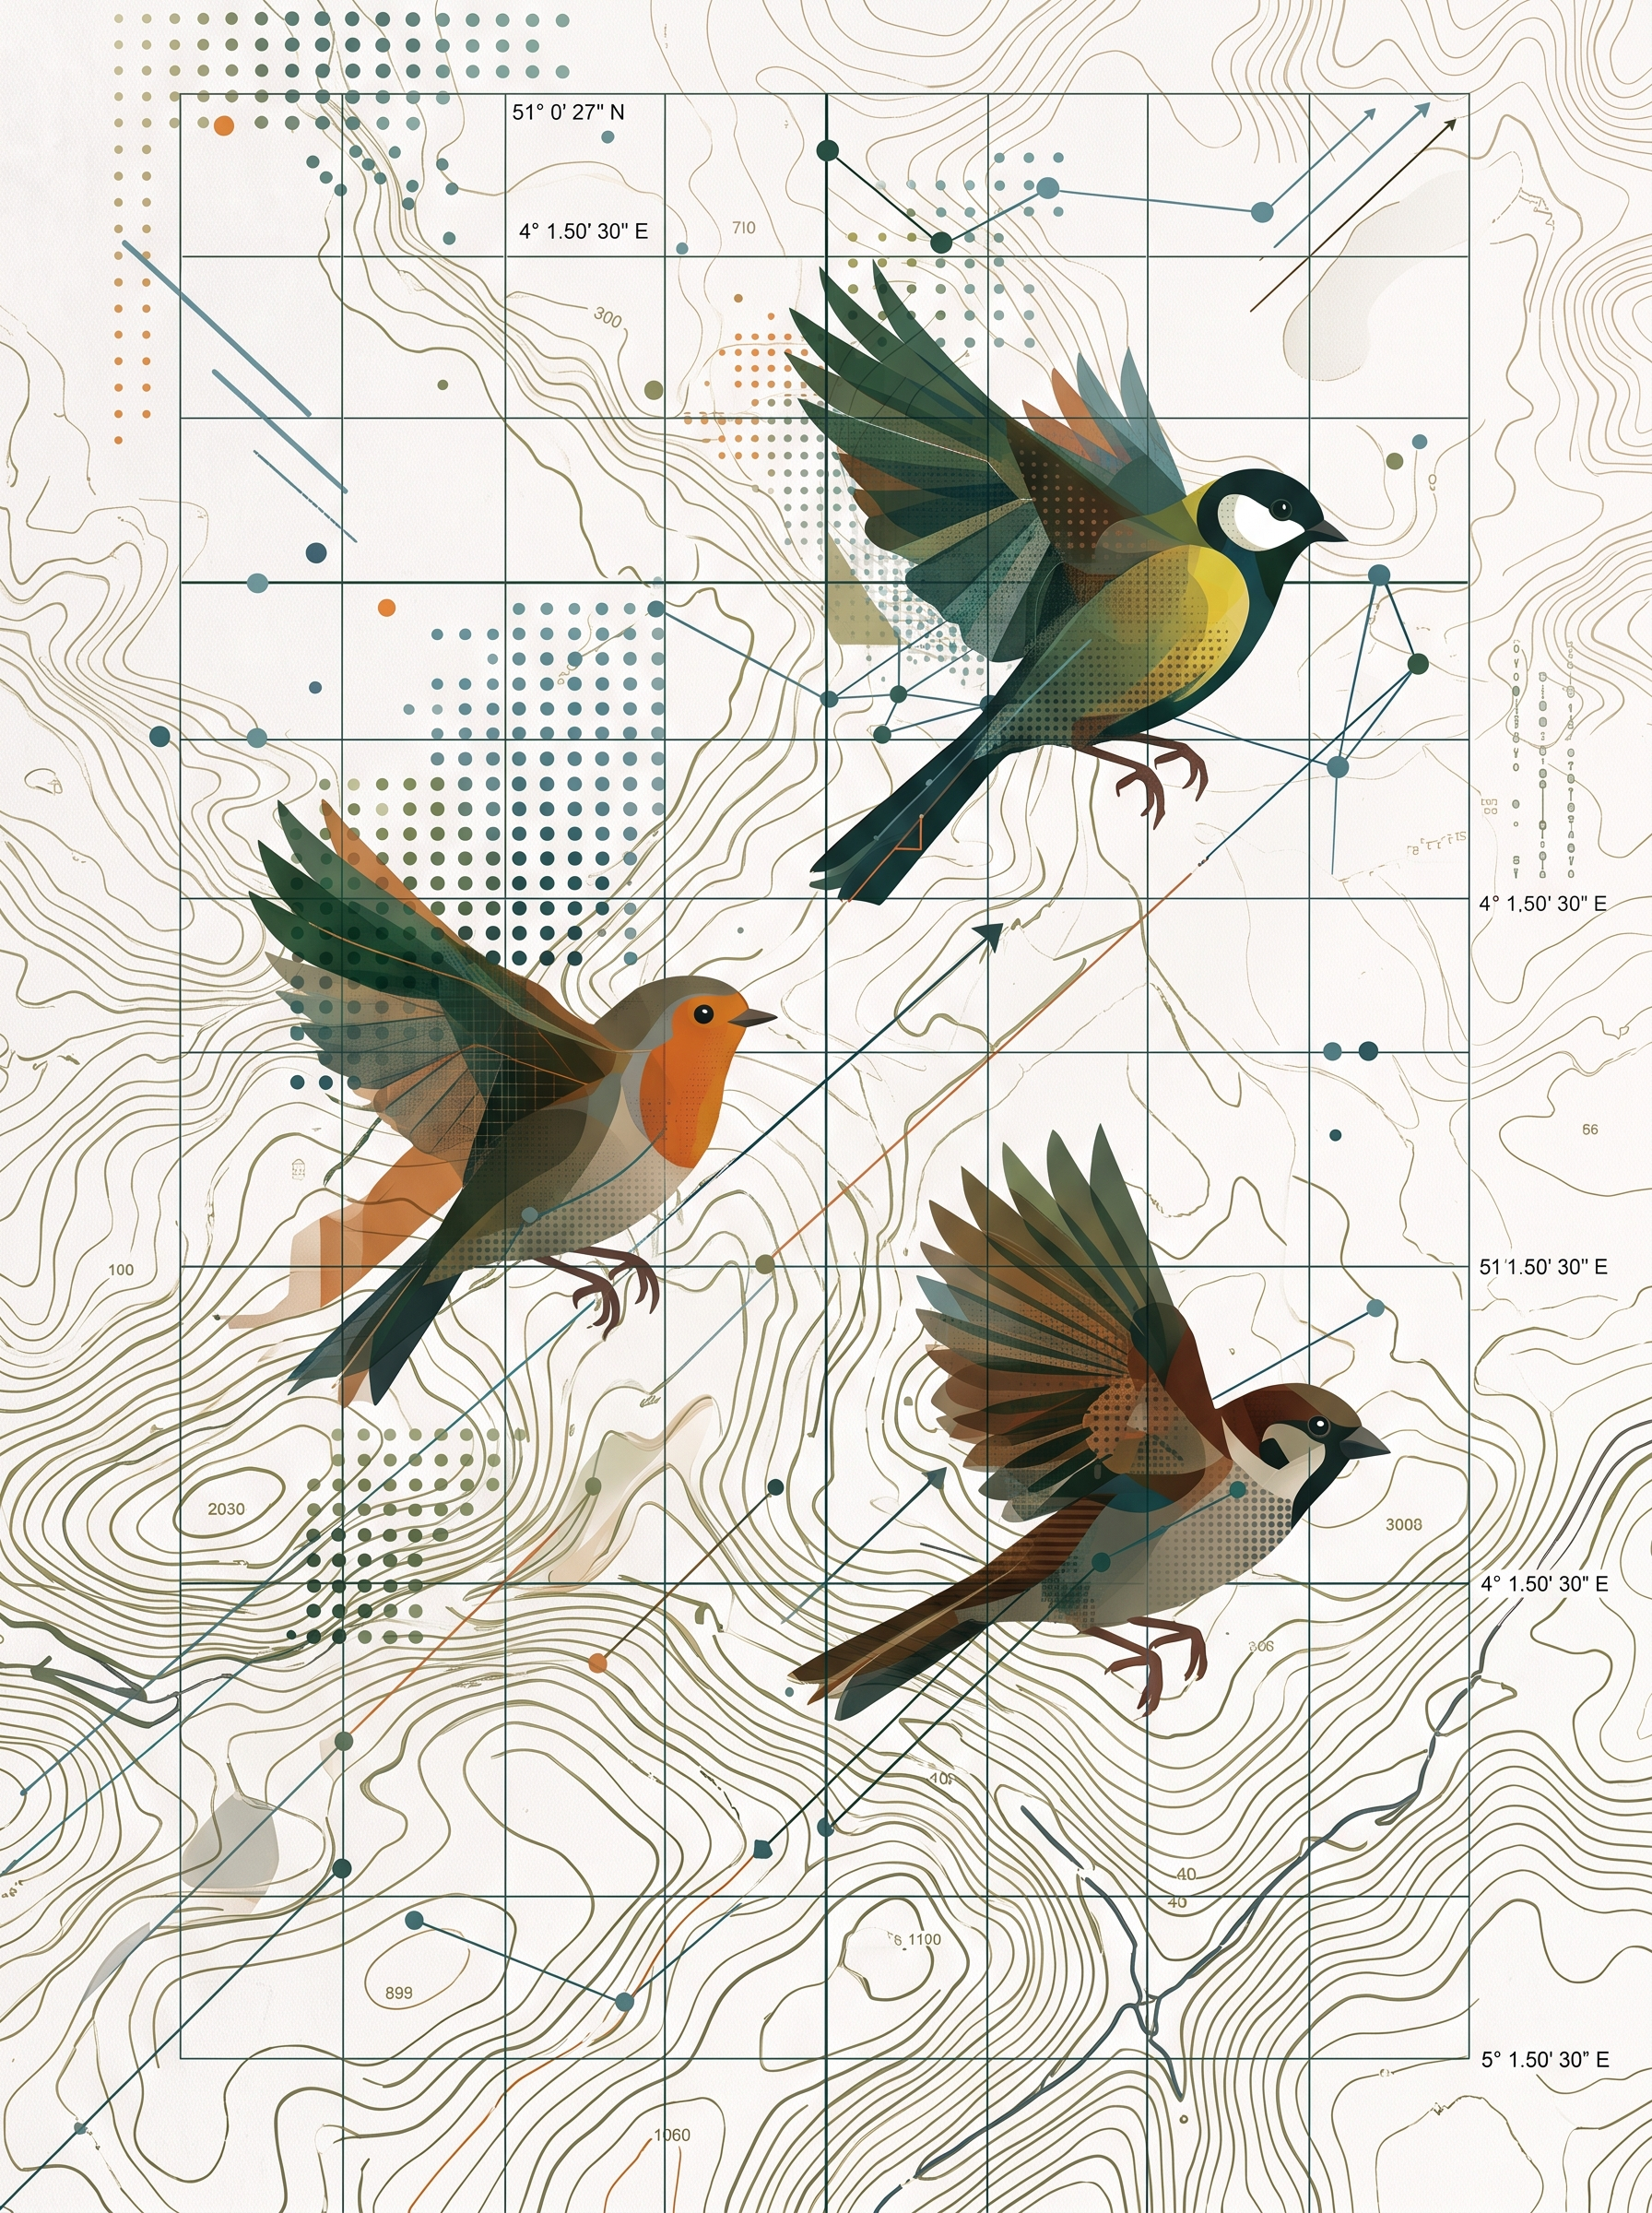
\includepdf[pages=1]{media/cover4.jpg}
\maketitle


\bookmarksetup{startatroot}

\chapter*{Preface}\label{preface}
\addcontentsline{toc}{chapter}{Preface}

\markboth{Preface}{Preface}

This is a Quarto book.

To learn more about Quarto books visit
\url{https://quarto.org/docs/books}.

\bookmarksetup{startatroot}

\chapter{STEEKPROEF}\label{steekproef}

Het huidig ABV meetnet is opgesteld door een steekproeftrekking uit UTM
1 x 1 km hokken. De regels van de trekking zijn gebaseerd op het
oppervlakteaandeel van een bepaald landgebruik op basis van de
Biologische Waarderingkaart (Vriens et al., 2011).

\begin{itemize}
\tightlist
\item
  Landbouw: minstens 80\% landbouw. 6311 hokken.
\item
  Urbaan: minstens 80\% urbaan. 416 hokken.
\item
  Bos: minstens 80\% bos. 319 hokken.
\item
  Suburbaan: minstens 80\% suburbaan. 201 hokken.
\item
  Heide en duin: minstens 20\% heide of duin. 199 hokken.
\item
  Moeras en water: minstens 20\% moeras en water. 137 hokken
\end{itemize}

In ieder gekozen hok worden er dan 6 metingen uitgevoerd per bezoek.
Voor verdere details verwijzen we naar (citatie). Bij deze steekproef
zijn er drie problemen.

\begin{itemize}
\tightlist
\item
  Een groot deel van Vlaander is niet beschikbaar voor de tellingen
  aangezien het Vlaams grondgebied zeer versnipperd is op ecologisch
  vlak. Indien men een uitspraak wil maken over de algemene broedvogels
  op Vlaams niveau, is het nodig om ook tellingen uit te voeren in de
  versnipperde gebieden.
\item
  De twee strata ``Heide en duin'' en ``Moeras en water'', worden nu
  geteld in hokken waarvan minimaal 20\% van het oppervlakte in het hok
  tot het respectievelijk strata toebehoort. De zes locaties waarin
  geteld worden kunnen in deze strata sterk verschillend zijn.
\item
  De locaties waren niet altijd even bereikbaar.
\end{itemize}

-\textgreater{} bewijs probleem 1 -\textgreater{} bewijs probleem 2
-\textgreater{} probleem 3 is anecdotisch

Het doel van het hernieuwde meetnet is om deze problemen te verheffen.

\section{FLEA}\label{flea}

In plaats van de Biologische Waarderingkaart vertrekken we nu vanuit de
Flanders Ecosystem Accounting (FLEA) kaarten, typologie niveau 2. Deze
kaarten worden gemaakt voor vorige en toekomstige jaren, we zullen de
steekproef hierdoor ook accurater kunnen aanpassen indien de ecosystemen
van bepaalde locaties veranderen.

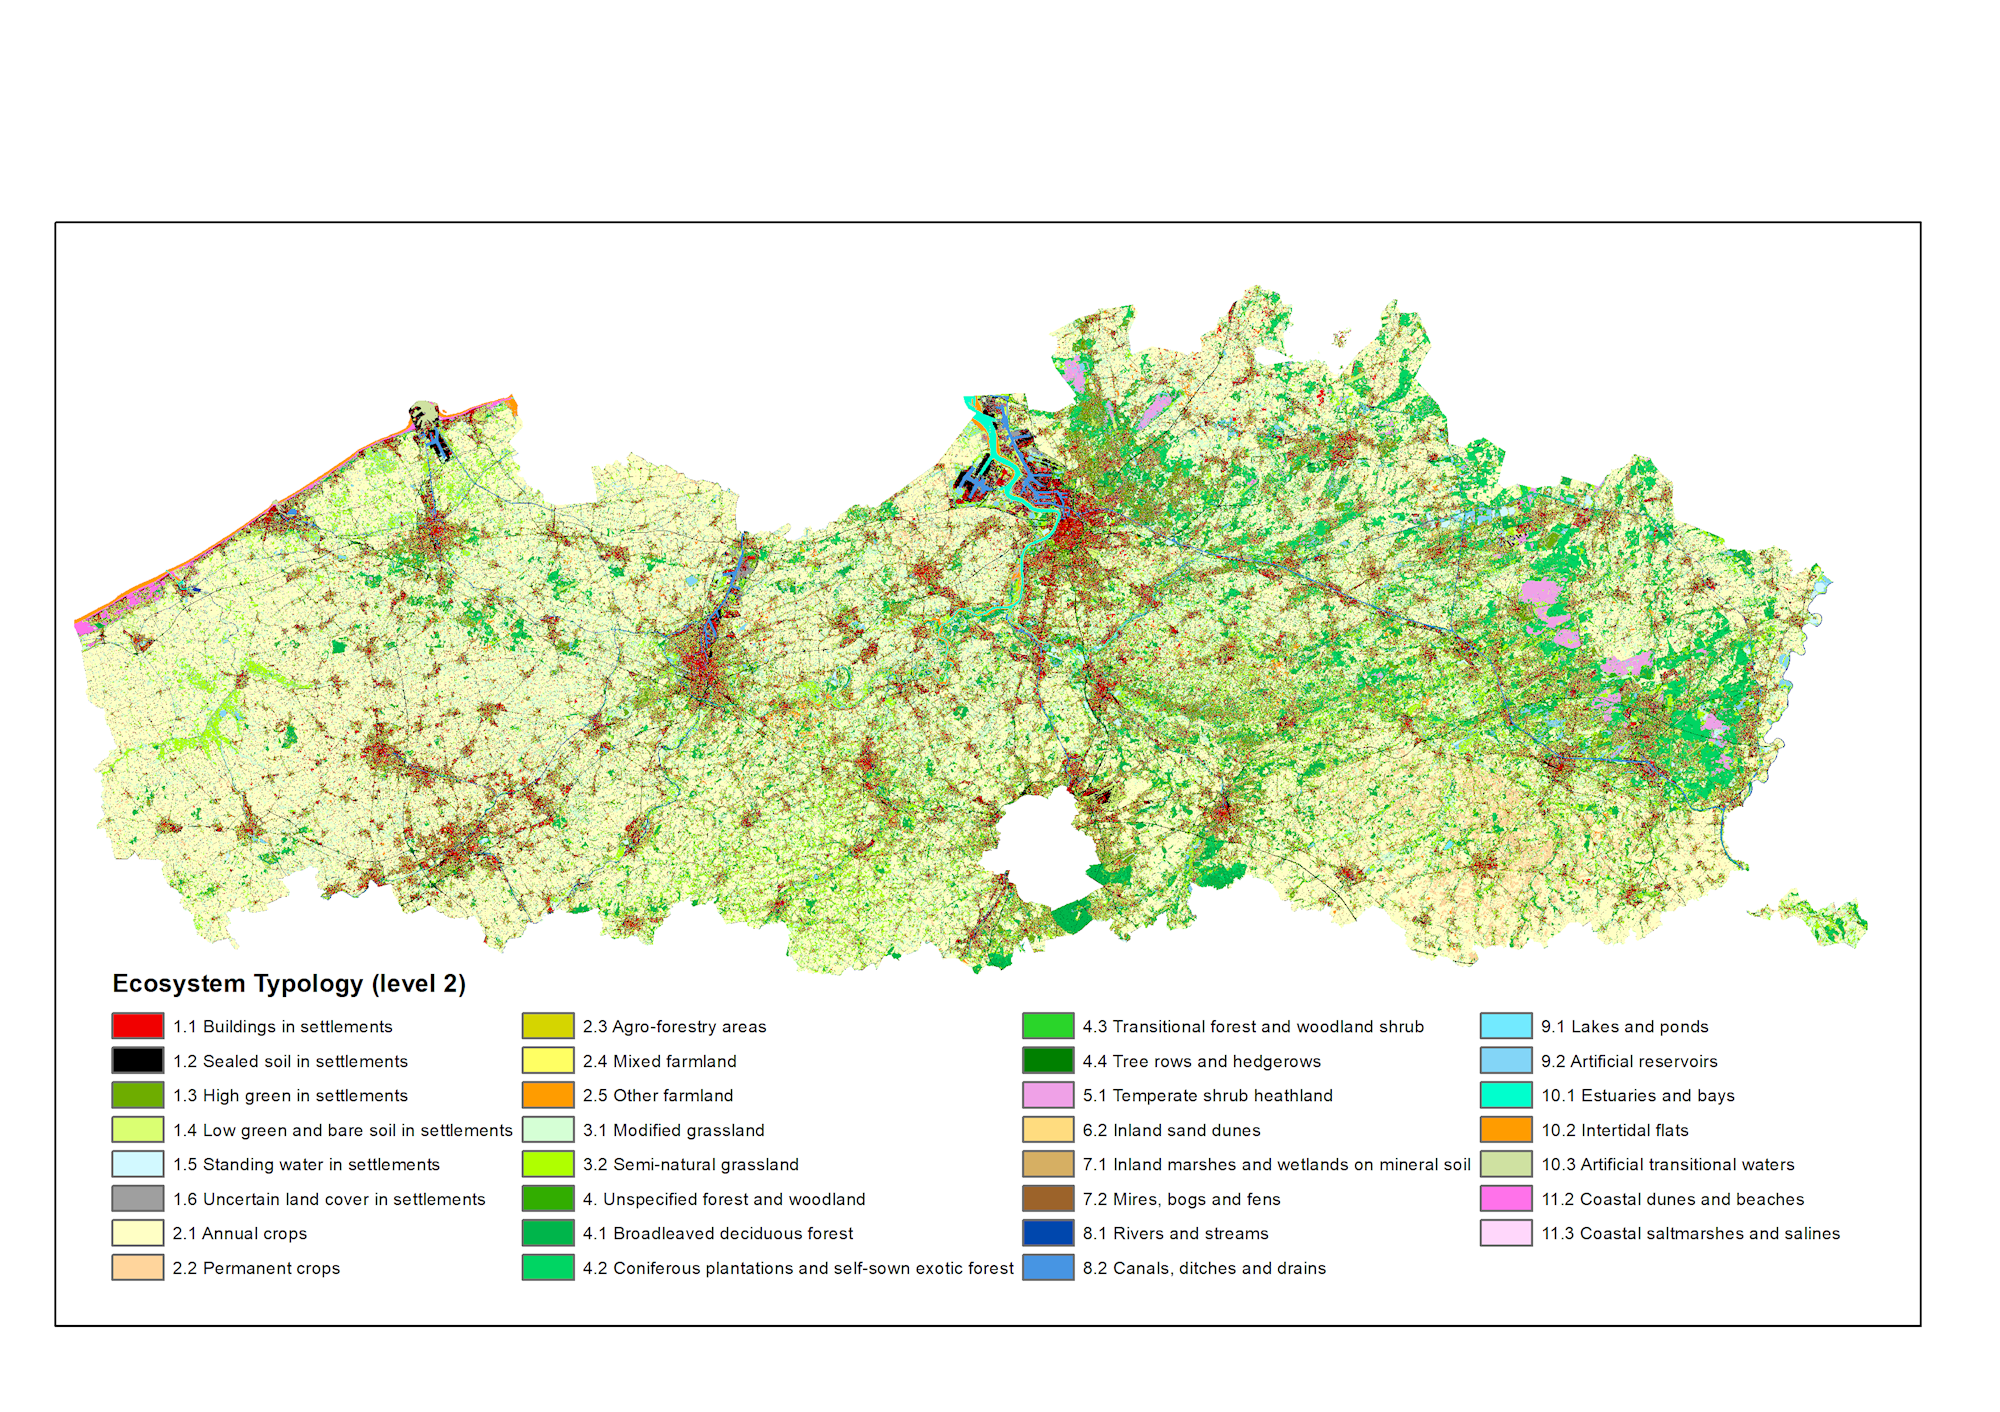
\includegraphics[width=\linewidth]{media/ecosystem_extent_2022_level2-1.png}

De FLEA kaart niveau 2 heeft 31 gedefiniëerde ecosysteem typologiën. De
steekproef om ieder verschillend type voldoende te samplen zou te groot
zijn. We hergrouperen deze typologiën in tien bredere strata en een
gemengde categorie:

\begin{itemize}
\tightlist
\item
  Urbaan: Bebouwing (1.1), verharde bodem (1.2) en onzekere
  bodembedekking binnen bebouwde ruimte (settlements = nederzettingen
  letterlijk vertaald) (1.6).
\item
  Urbaan groen: Hoog groen (1.3) en laag groen/onbedekte bodem binnen
  bebouwde ruimte (1.4).
\item
  Akker: Alle agrarische typen, waaronder eenjarige gewassen (2.1),
  permanente gewassen (2.2), agroforestry (2.3), gemengde landbouw (2.4)
  en overige landbouwgronden (2.5).
\item
  Grasland: Intensief/beheerd grasland (3.1) en halfnatuurlijk grasland
  (3.2).
\item
  Bos: Ongespecificeerd bos (4.0), loofbos (4.1), naaldbos en exoten
  (4.2), overgangszone bos/struikgewas (4.3) en bomenrijen/heggen (4.4).
\item
  Duinen en heide: heide (5.1), landduinen (6.2), kustduinen/stranden
  (11.2) en schorren/zoutmoerassen (11.3).
\item
  Moeras: Binnenlandse moerassen op minerale bodem (7.1) en
  veengebieden/venen (7.2).
\item
  Stilstaand en lopend water: Stilstaand water in bebouwde ruimte (1.5),
  rivieren en beken (8.1), kanalen en grachten (8.2), meren en vijvers
  (9.1) en kunstmatige reservoirs (9.2).
\item
  Estuarium: Estuaria en baaien (10.1).
\item
  Getijdengebied en overgangswater: getijdenplaten (10.2) en kunstmatig
  overgangswater (10.3).
\item
  Gemengd: toegewezen na het berekenen van de focal window (zie
  hoofdstuk focal window)
\end{itemize}

\section{FOCAL WINDOW}\label{focal-window}

Voor het focal window gebruikten we een gaussiaanse verdeling waarbij
het centrum het grootste gewicht krijgt. De direct omgeving waar de
vrijwilleger tellingen uitvoert, is dus het belangrijkste om de strata
aan te wijzen. Maar we houden op deze manier nog steeds rekening met de
verdere omgeving.

De keuze van de gaussiaanse distributie is gekozen door te vergelijken
met een d van 50m,100m en 200m. We hebben gekozen voor 100m door de
vraag om bossen van grootte X nog te kunnen behouden terwijl we kleinere
weglaten. Met een kleinere cirkel tellen we alle kleine bossen mee,
terwijl een cirkel van 200 m enkel de grootste bossen meetelt.

insert cijfers

Gewichtsverdeling van het gaussian focal window op een raster van 10 ×
10 m. Het kleurgradiënt geeft het gewicht per pixel weer, waarbij de
pixels in het centrum het hoogste gewicht dragen en de invloed afneemt
naarmate de afstand tot het centrum toeneemt.

TODO: cijfers met betrekking tot het aantal patches hiernaast zetten.

\begin{figure}[H]

{\centering \pandocbounded{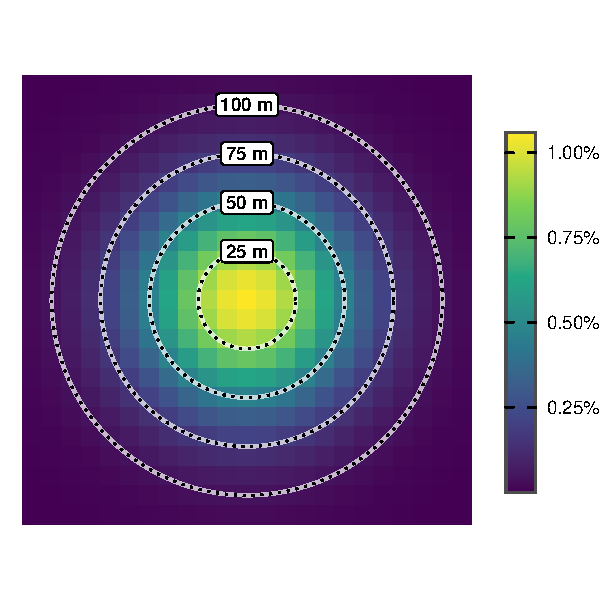
\includegraphics[keepaspectratio]{source/steekproef_files/figure-pdf/focal-window-plot-1.pdf}}

}

\caption{Gaussiaans focal window met de hoogste gewichten in het centrum
en afnemende invloed naar buiten.}

\end{figure}%

\begin{itemize}
\tightlist
\item
  uitleg over de gaussian focal window (definieer, hoe, waarom, impact)

  \begin{itemize}
  \tightlist
  \item
    waarom 100m en niet meer of minder (patch analyse tonen)
  \item
    Figuur met betrekking tot
  \item
    Volledige cijfer uitzetten, hoeveel van iedere strata
  \end{itemize}
\end{itemize}

Een focal window van radius GaussianRadius 100m rond 100m met een
gaussian distributie met sigma X als weights. We lopen dit over iedere
UTM 10 x 10m pixels van FLEA kaart (todo: link). Nieuwe strata, vanuit
de FLEA kaart ook, samengevoegd. Rechtstreeks van hieruit samplen.

\section{OSM}\label{osm}

\begin{itemize}
\tightlist
\item
  eerdere problematiek van bereikbaarheid

  \begin{itemize}
  \tightlist
  \item
    oplossing: openstreetmap -\textgreater{} buffer (beperk beweging to
    binnen de buffer, indien niet mogelijk dan verwijderen we dit punt)
  \end{itemize}
\end{itemize}

\bookmarksetup{startatroot}

\chapter{STEEKPROEF}\label{steekproef-1}

\begin{itemize}
\item
  uitleg vertrekpunt van de kaart (FLEA)
\item
  uitleg over de gaussian focal window (definieer, hoe, waarom, impact)

  \begin{itemize}
  \tightlist
  \item
    waarom 100m en niet meer of minder (patch analyse tonen)
  \item
    Volledige cijfer uitzetten, hoeveel van iedere strata
  \end{itemize}
\end{itemize}

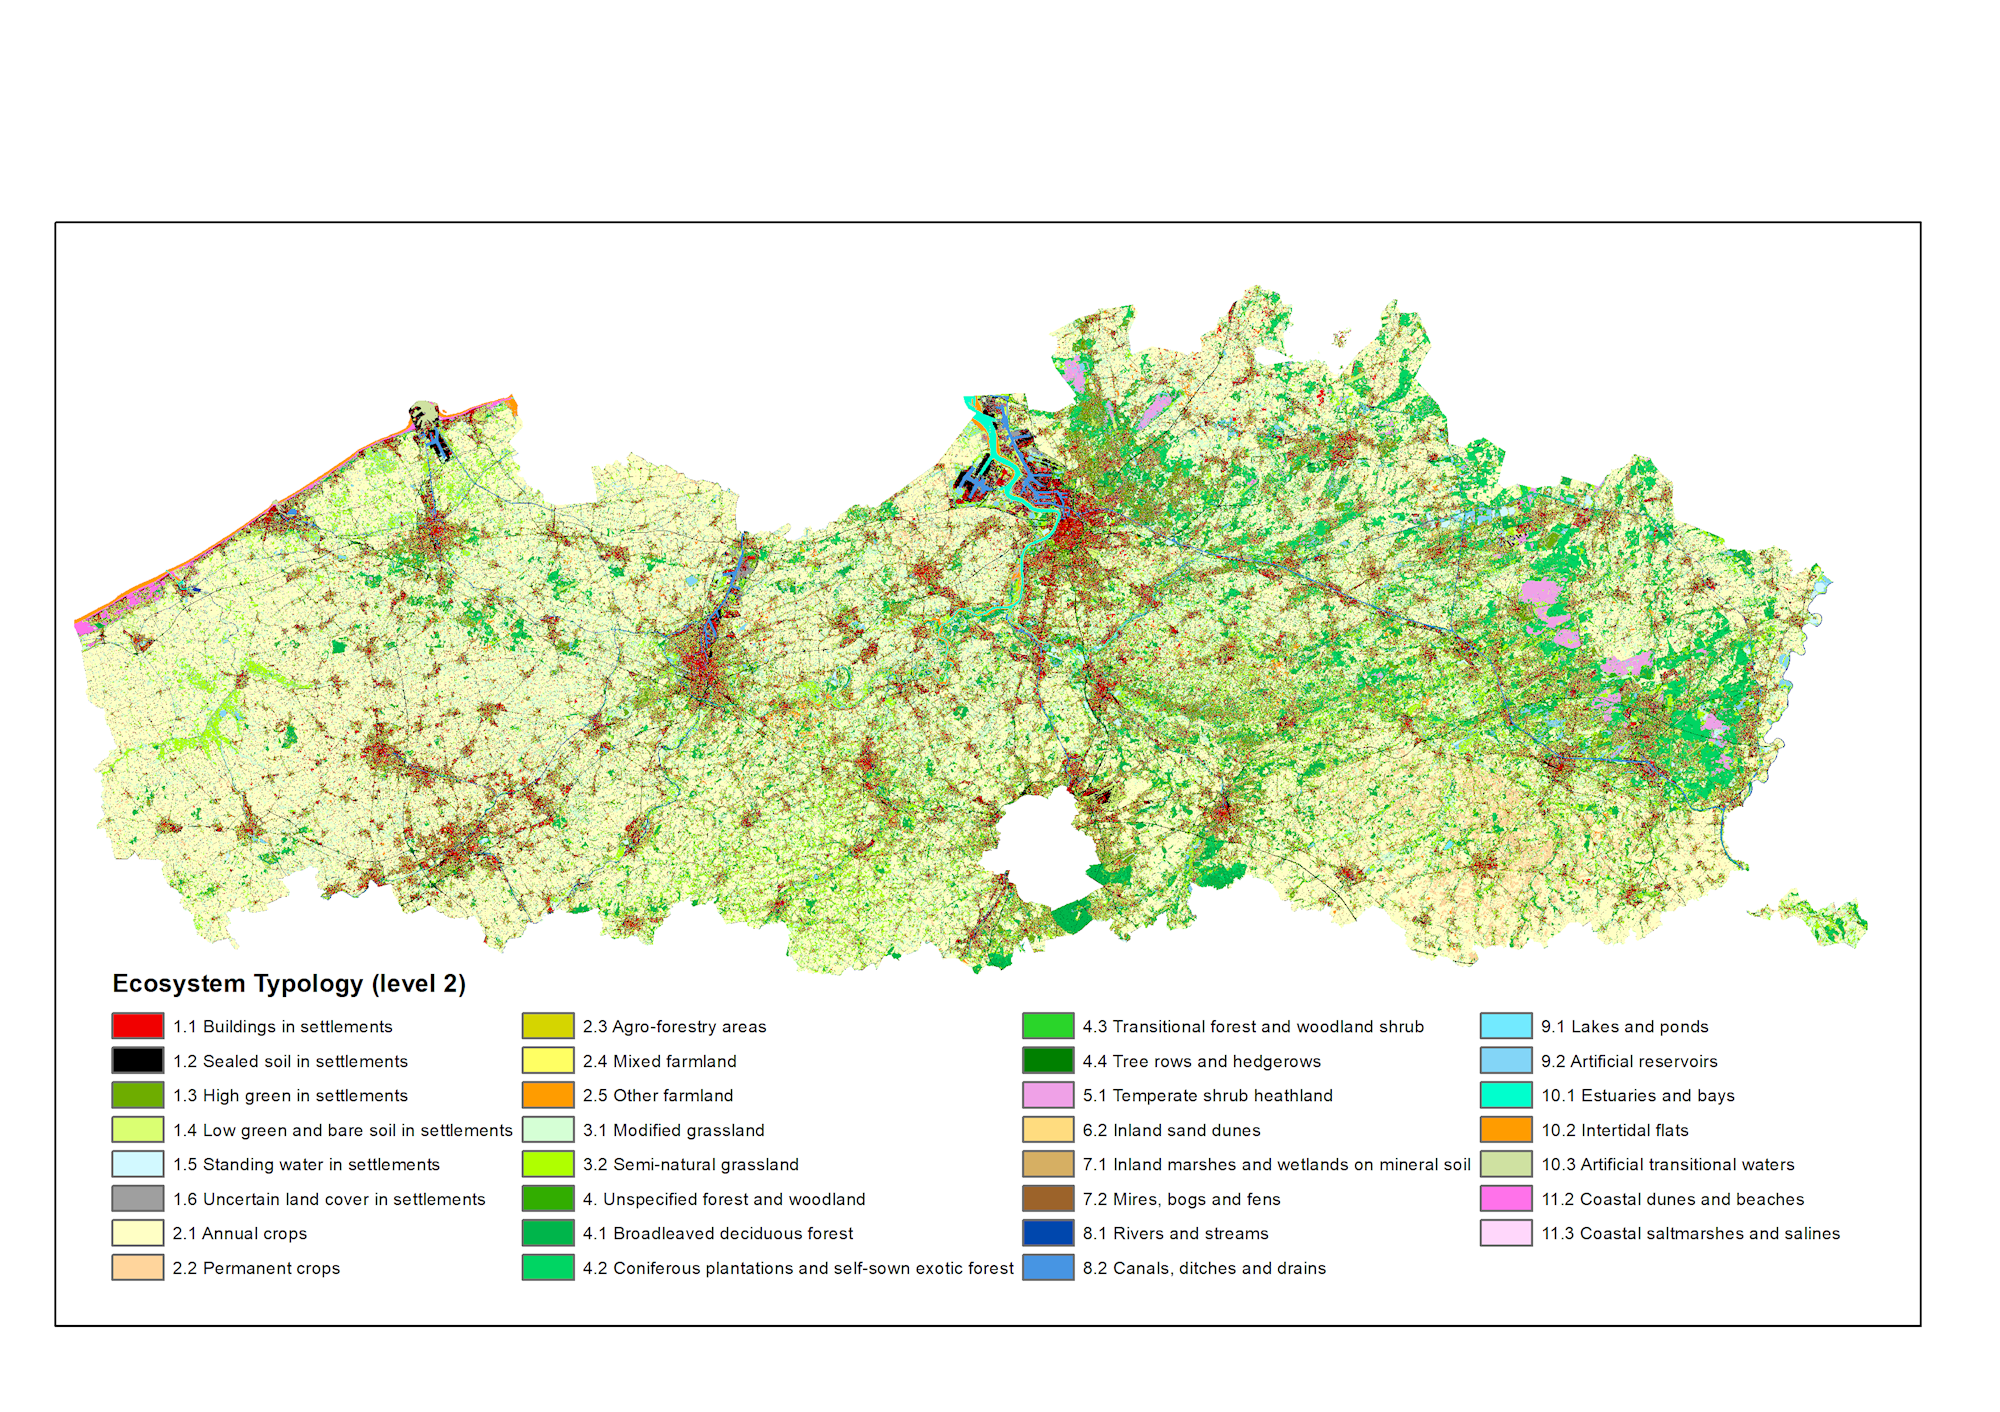
\includegraphics[width=\linewidth]{media/ecosystem_extent_2022_level2-1.png}

\begin{itemize}
\tightlist
\item
  eerdere problematiek van bereikbaarheid

  \begin{itemize}
  \tightlist
  \item
    oplossing: openstreetmap -\textgreater{} buffer (beperk beweging to
    binnen de buffer, indien niet mogelijk dan verwijderen we dit punt)
  \end{itemize}
\end{itemize}

\section{PATCH ANALYSE}\label{patch-analyse}

\section{OPEN STREETMAP ANALYSE}\label{open-streetmap-analyse}

\section{POWER ANALYSE}\label{power-analyse}

\bookmarksetup{startatroot}

\chapter{VERWERKING VAN DE GEGEVENS}\label{verwerking-van-de-gegevens}

\begin{itemize}
\item
  De flea kaarten worden herwerkt van de vorige jaren
\item
  Dezelfde modellen gebruiken, voorlopige vergelijking van de modellen
  uitschrijven (kijk hoe nuttig dit is, toont gewoon aan dat er geen al
  te grote veranderingen zouden moeten zijn)
\end{itemize}

\bookmarksetup{startatroot}

\chapter{TRENDBEREKENING}\label{trendberekening}

\begin{itemize}
\tightlist
\item
  Opgelet voor veranderende weights van de data per FLEA kaart.
\end{itemize}

\bookmarksetup{startatroot}

\chapter{VOORSTELLING VAN DE
GEGEVENS}\label{voorstelling-van-de-gegevens}

\begin{itemize}
\tightlist
\item
  Exact hetzelfde noormaal gezien
\end{itemize}

\bookmarksetup{startatroot}

\chapter{REPRODUCEERBAARHEID EN TRACEERBAARHEID VAN DE
GEGEVENSVERWERKING}\label{reproduceerbaarheid-en-traceerbaarheid-van-de-gegevensverwerking}

\begin{itemize}
\tightlist
\item
  Verduidelijken dat we het eerdere script zullen runnen op de vorige
  aangemaakte kaarten. Deze passen we dan aan.
\item
  Manier van reproduceerbaarheid en traceerbaarheid houden we exact
  hetzelfde denk ik.
\end{itemize}

\bookmarksetup{startatroot}

\chapter{Summary}\label{summary}

In summary, this book has no content whatsoever.

\bookmarksetup{startatroot}

\chapter*{References}\label{references}
\addcontentsline{toc}{chapter}{References}

\markboth{References}{References}

\protect\phantomsection\label{refs}




\end{document}
